\chapter{Analisis}
\label{chap:analisis}

Bab ini membahas tentang analisis kebutuhan Sharif Judge yang diperlukan oleh Teknik Informatika. Kebutuhan-kebutuhan tersebut didapat dari daftar isu repositori Sharif Judge di \textit{GitHub} dan dari para dosen pengguna Sharif Judge. Hasil dari analisis kebutuhan tersebut dicatat ke dalam \textit{Google Sheets} dan didiskusikan dengan dosen pembimbing. Selain analisis kebutuhan, pada bab ini juga akan dibahas solusi yang ditawarkan untuk memenuhi kebutuhan tersebut. Berikut hasil diskusi peniliti bersama dosen pembimbing yang dicatat ke dalam \textit{Google Sheets}. 

\begin{figure}[H]
	\centering  
	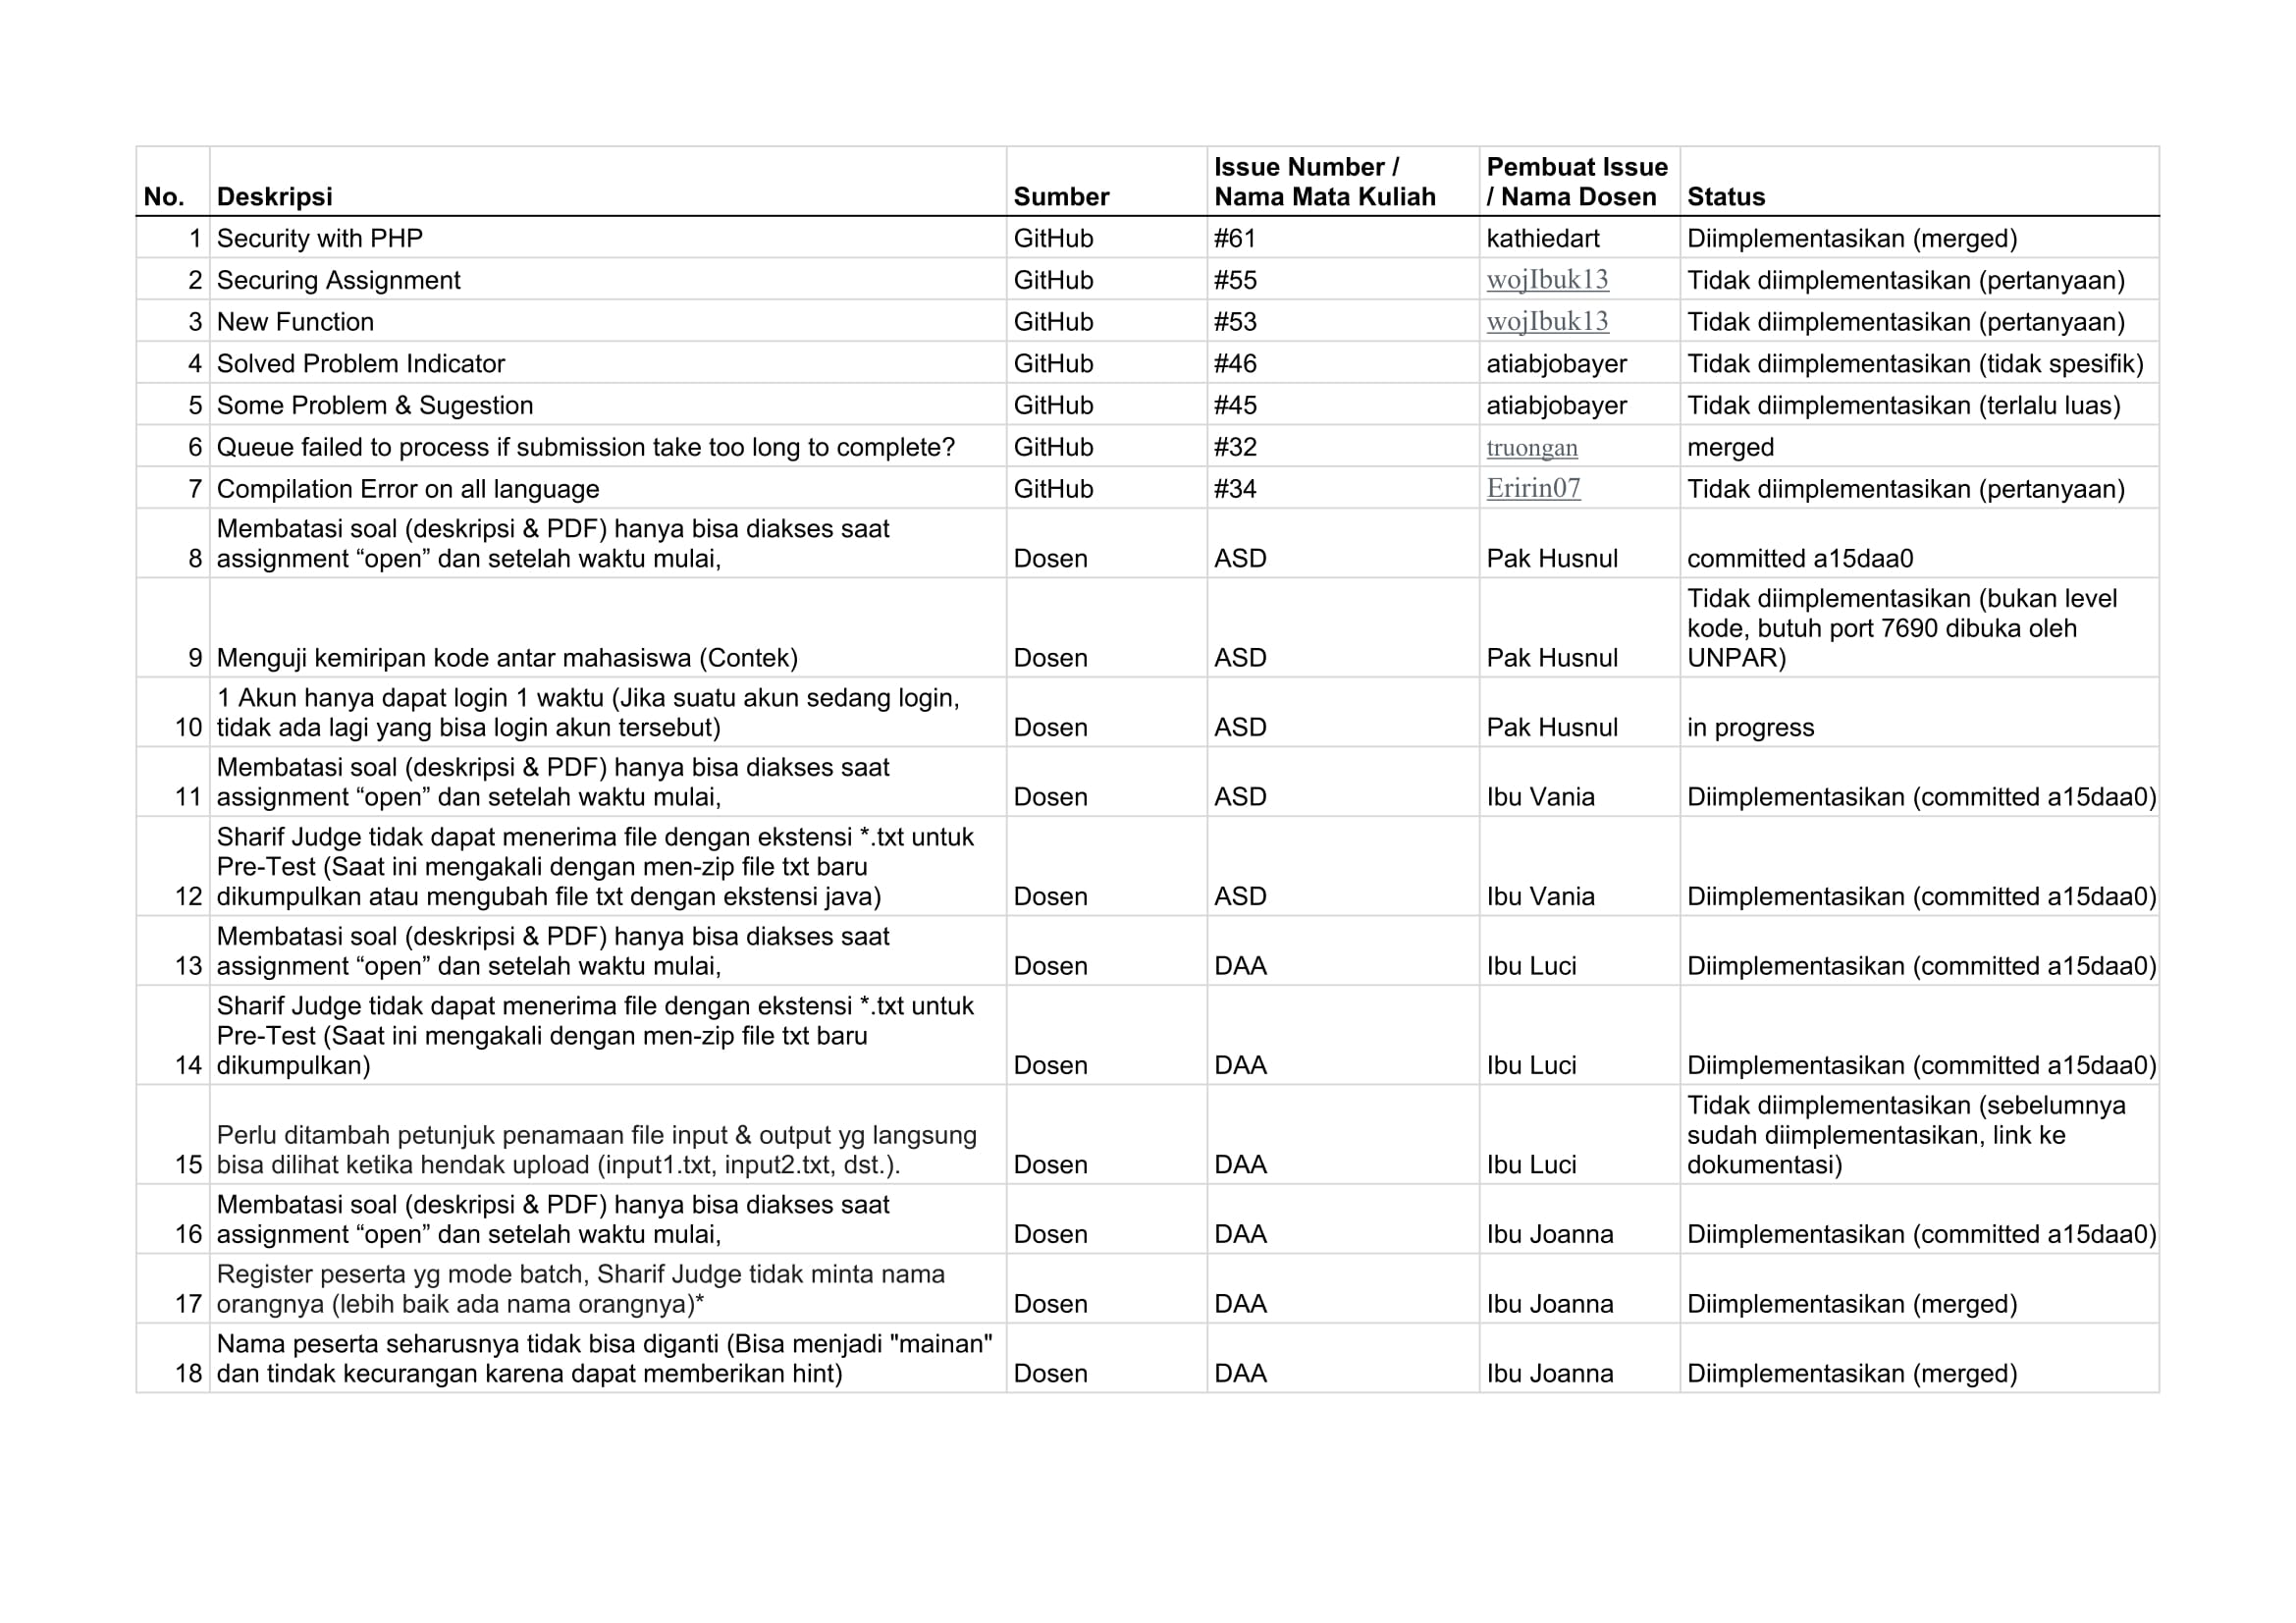
\includegraphics[scale=0.2]{pdf1}
	
	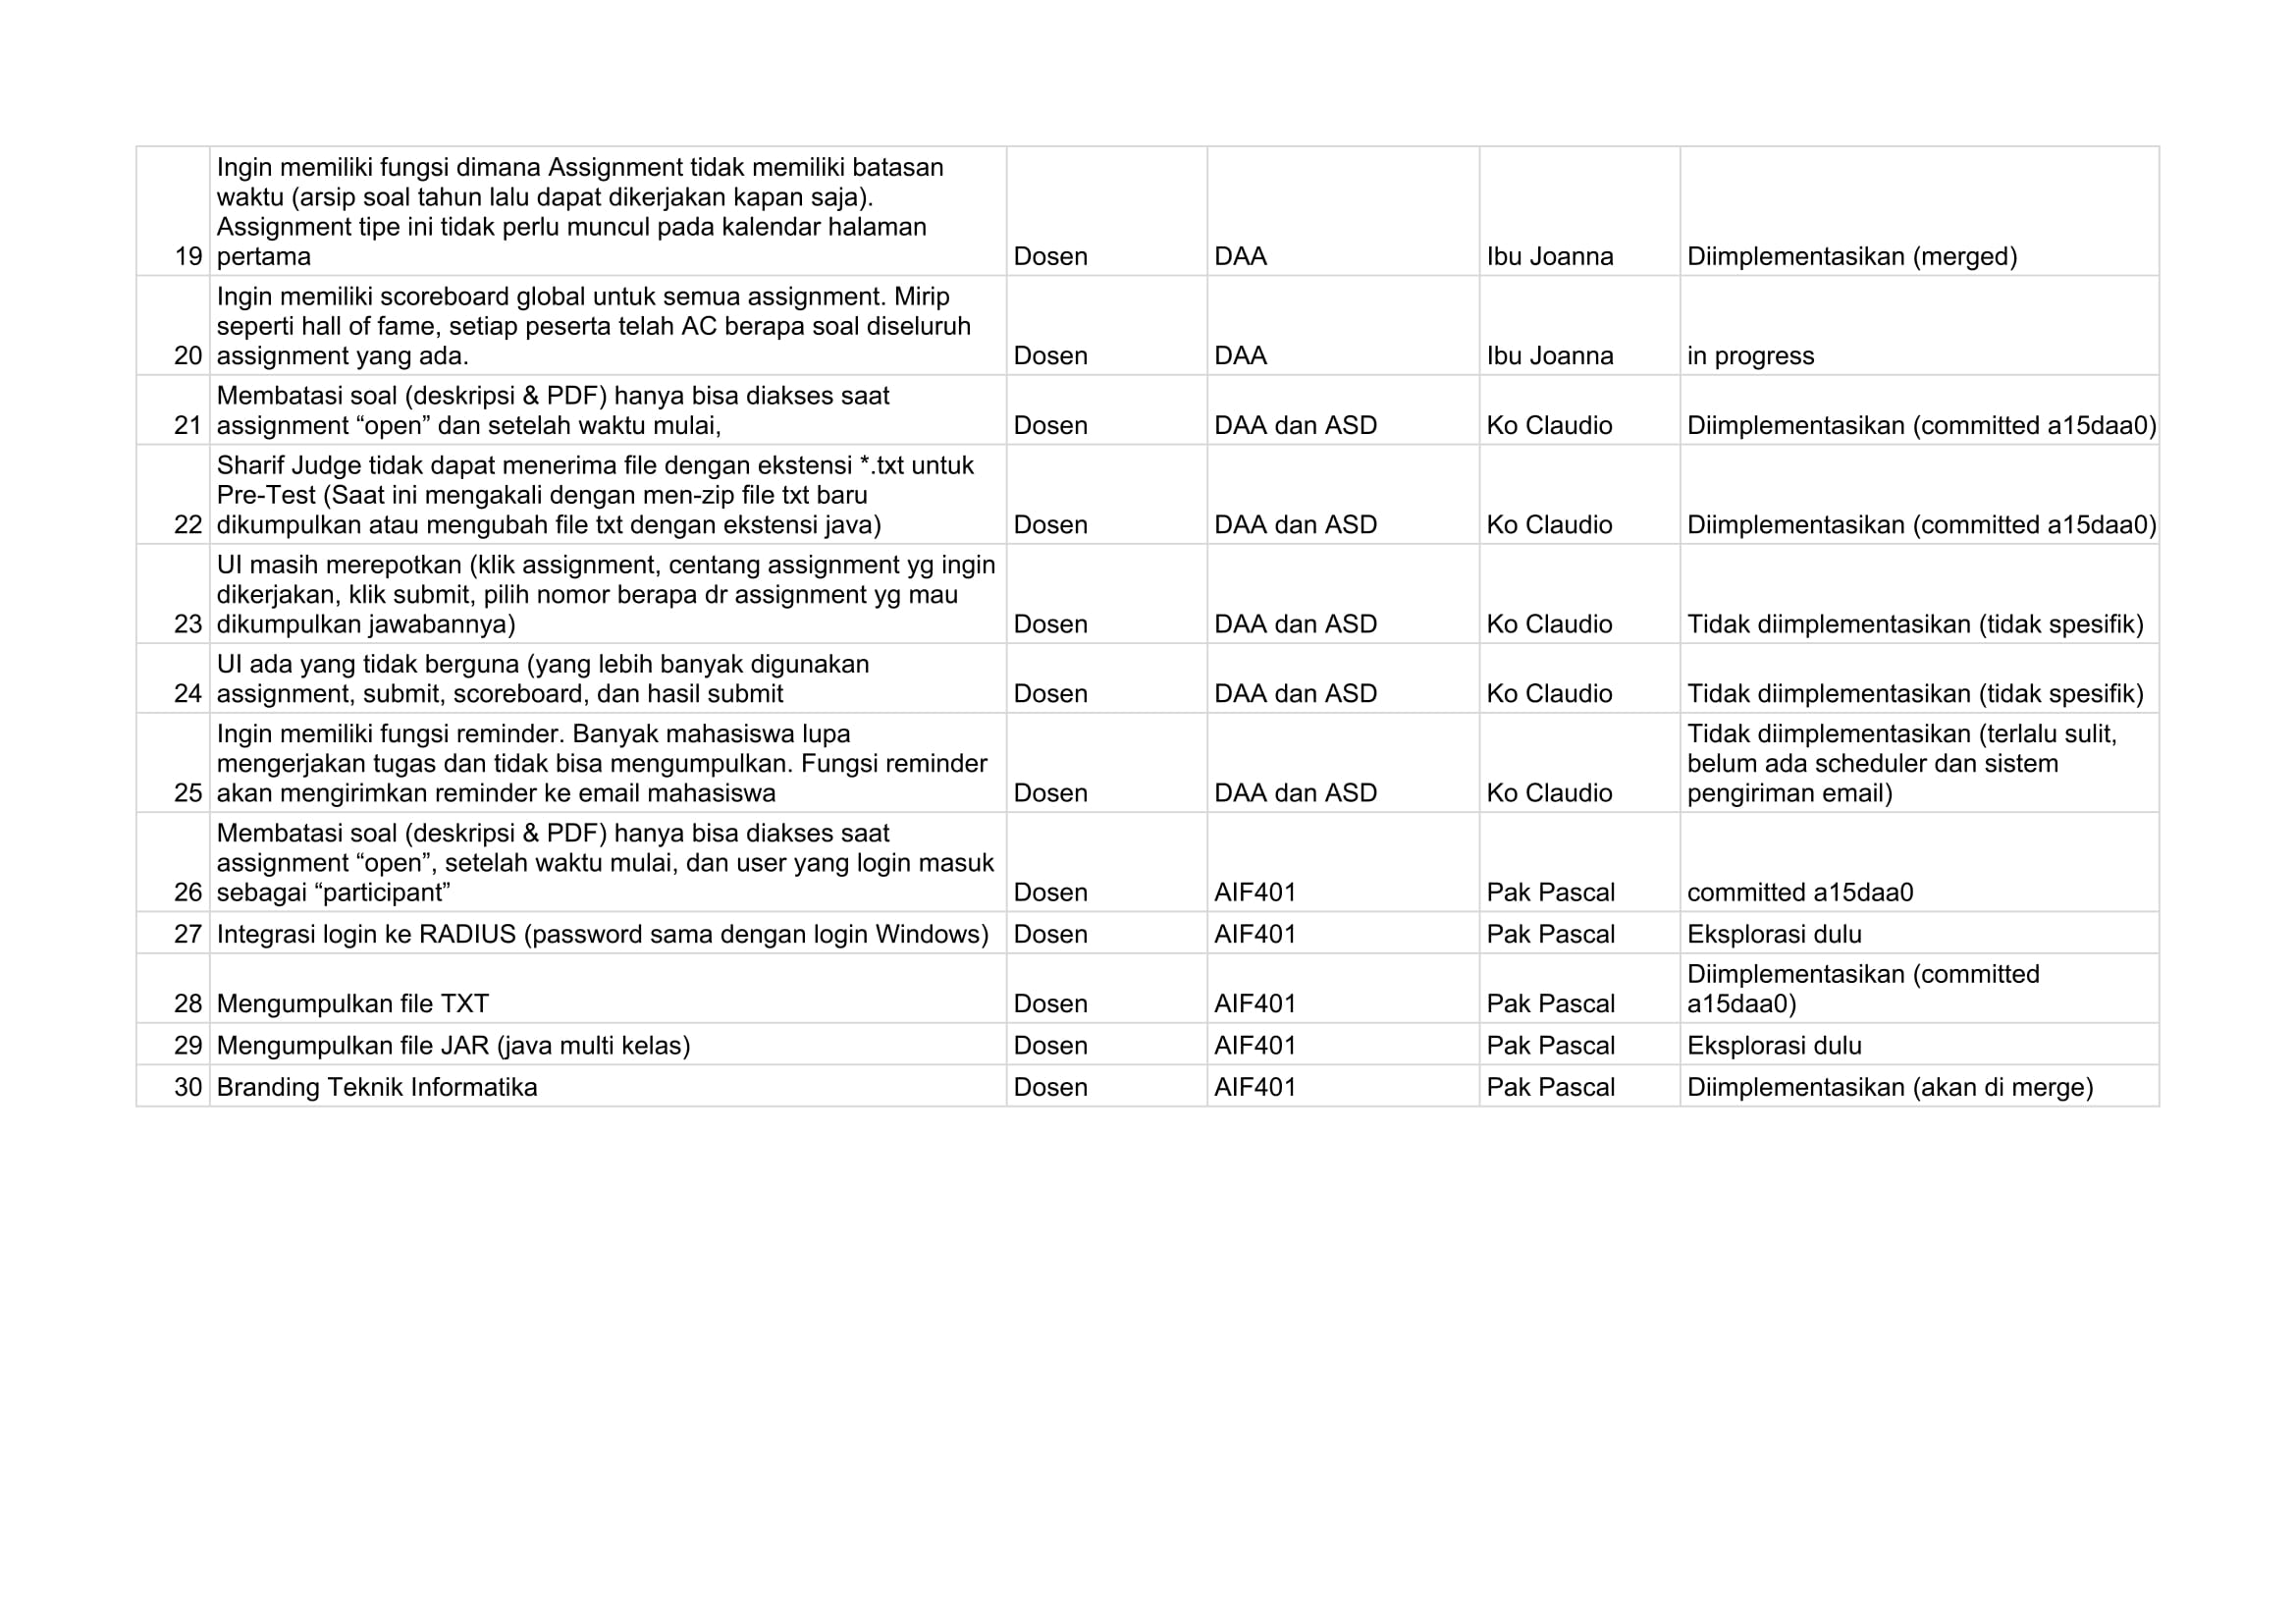
\includegraphics[scale=0.2]{pdf2}
\end{figure}


\section{Analisis Kebutuhan dari Daftar Isu Repositori Sharif Judge   \textit{GitHub}}
\label{sec:analisisgithub} 
Analisis dilakukan dengan menganalisa setiap isu terbuka yang ada pada repositori. Dari analisa setiap isu tersebut, didapatkan beberapa pertanyaan dan usulan pengembangan. Beberapa isu yang memiliki usulan pengembangan akan dijadikan pertimbangan untuk mengembangkan Sharif Judge.

\subsection{\textit{Security with PHP}}
Isu ini dibuat oleh pengguna \textit{GitHub} dengan username \textit{danwdart}. Pada isu tersebut dikatakan bahwa seseorang pengguna Sharif Judge dapat mengubah parameter PHP \textit{shell\_exec()} yang mengakibatkan pengeksekusian kode bisa dilakukan secara sewenang-wenang. Solusi yang ditawarkan untuk mengatasi hal diatas adalah mengganti penggunaan PHP \textit{shell\_exec()} dengan method lain. Contohnya seperti perintah \textit{shell\_exec("rm ...")} yang memiliki fungsi untuk menghapus sebuah file. Perintah tersebut dapat diganti menggunakan method \textit{unlink()} yang memiliki fungsi sama yaitu menghapus sebuah file.
%Hal tersebut dapat dicegah dengan cara mengubah perintah shell\_exec("rm ...") dengan method \textit{unlink()}.
	
\subsection{\textit{Queue failed to process if submission take too long to complete?}}
Isu ini dibuat oleh pengguna \textit{GitHub} dengan username \textit{truongan}. Pada isu tersebut dikatakan bahwa assignment yang memiliki masalah dengan test case besar akan menyebabkan \textit{submission status} menjadi \textit{pending}. User \textit{truongan} memperkirakan hal diatas terjadi dikarenakan \textit{database connection times out}. Solusi yang ditawarkan untuk mengatasi hal diatas adalah menambahakan \textit{method reconnect database}. \textit{Method reconnect database} akan menghubungkan kembali database ketika terjadi kasus seperti diatas.
% Untuk mengatasi masalah tersebut diperlukan method reconnect database pada file \textit{Queueprocess.php}.

\section{Analisis Kebutuhan dari Dosen Pengguna Sharif Judge}
\label{sec:analisisdosen} 
Analisis kebutuhan dari para dosen pengguna Sharif Judge dilakukan dalam bentuk wawancara secara langsung dan melalui email. Dosen-dosen yang telah diwawancarai antara lain:
\begin{enumerate}
	\item Bapak Husnul Hakim
	\item Bapak Claudio Franciscus
	\item Ibu Vania Natali
	\item Ibu Luciana Abednego
	\item Ibu Joanna Helga
\end{enumerate}
Dari hasil wawancara didapatkan beberapa kebutuhan yang sama dari setiap dosen pengguna Sharif Judge. 

\subsection{Menguji kemiripan kode antar mahasiswa}
Perangkat lunak Sharif Judge terkini sudah memiliki fitur untuk menguji kemiripan kode antar peserta dengan menggunakan Moss (\textit{Measure Of Software Similarity}). Moss adalah sistem otomatis untuk mendeteksi kemiripan program. Aplikasi Moss telah berkembang dari tahun 1994 hingga sekarang. Algoritma yang digunakan pada aplikasi Moss sangat efektif dibandingkan algoritma deteksi kecurangan lainnya \footnote{Alex Aiken, "A System for Detecting Software Similarity" Plagiarism Detection. \textit{http://theory.stanford.edu/~aiken/moss/} (diakses 25 Februari 2018)}. Namun untuk sekarang ini, Moss tidak dapat digunakan karena aplikasi Moss membutuhkan port 7690 yang diblok oleh UNPAR. Oleh sebab itu, kebutuhan ini tidak diimplementasikan.

\subsection{Satu Akun hanya dapat login satu waktu}
Para peserta Sharif Judge dapat login menggunakan akunnya di beberapa komputer. Peserta yang mengetahui user dan password peserta lain dapat dengan mudah login ke Sharif Judge. Hal tersebut sering dijadikan celah bagi beberapa peserta untuk melakukan tindak kecurangan. Peserta yang sudah login menggunakan akun peserta lainnya, dapat melihat dan menyalin kode yang telah dikumpulkan ke Sharif Judge. Tindak kecurangan ini sering terjadi pada saat kuis maupun ujian. Bapak Husnul Hakim menginginkan perangkat lunak Sharif Judge dimana akun para peserta hanya dapat login satu waktu. Jika sebuah akun telah login di satu komputer, maka akun tersebut tidak dapat login di komputer lainnya. Diharapkan dengan adanya fitur tersebut dapat menekan jumlah tindak kecurangan yang terjadi. \\
Solusi yang ditawarkan untuk mengurangi tingkat kecurangan seperti diatas yaitu membuat halaman baru yang berisikan \textit{logs} username yang berhasil login ke Sharif Judge. Halaman logs tersebut akan mencatat username yang login menggunakan ip berbeda dalam waktu dibawah 24 jam. Dengan adanya halaman Logs ini, para dosen dapat memantau username yang login pada dua tempat berbeda.	

\subsection{Perlu ditambah petunjuk penamaan file input dan output}
Dalam membuat sebuah assignment pada perangkat lunak Sharif Judge terdapat file test case yang harus disertakan. File test case yang disertakan memiliki beberapa ketentuan. Beberapa ketentuan tersebut seperti struktur direktori dan penamaan dalam file test case. Pada halaman add assignment telah disediakan link menuju dokumentasi Sharif Judge di \textit{GitHub} yang menjelaskan ketentuan dalam menyertakan file test case. Ketentuan tersebut harus terpenuhi agar sebuah assignment dapat berjalan dengan baik. Oleh sebab itu, kebutuhan ini tidak diimplementasikan.

%\subsection{UI masih merepotkan}

%\subsection{UI ada yang tidak berguna}

\subsection{Sharif Judge diharapkan memiliki fungsi reminder}
Setiap assignment pada perangkat lunak Sharif Judge memiliki batas pengumpulan. Jika assignment telah melewati batas pengumpulan maka para peserta tidak dapat mengumpulkan tugasnya. Banyak peserta sering kali lupa untuk mengerjakan assignment dan pada akhirnya melewati batas pengumpulan. Bapak Claudio Fransiscus menginginkan perangkat lunak Sharif Judge yang memiliki fitur reminder. Fitur reminder akan mengirimkan email ke setiap peserta yang berisikan peringatan bahwa ada assignment yang harus diselsaikan. Namun kebutuhan ini belum dapat diimplementasikan karena masih belum ada sistem \textit{scheduller} dan tingkat kesulitan yang terlalu tinggi.

\subsection{Membatasi soal (deskripsi \& PDF) hanya bisa diakses saat assignment "open" dan setelah waktu mulai}
Kebutuhan ini merupakan salah satu kebutuhan yang paling banyak disebut oleh para dosen pengguna Sharif Judge. Perangkat lunak Sharif Judge terkini masih belum dapat memenuhi kebutuhan diatas. Para peserta dapat mengunduh deskripsi soal \& PDF sebelum waktu assignment dimulai. Untuk menangani hal tersebut para dosen harus mengunggah file PDF tepat pada saat assignment dimulai. \\
Solusi yang ditawarkan untuk memenuhi kebutuhan diatas yaitu membatasi soal agar dapat diunduh pada saat assignment "open" dan setelah waktu mulai. Jika ada peserta yang mencoba untuk mengunduh soal (deskripsi \& PDF) pada saat assignment belum dimulai, maka akan muncul pesan error \textit{"Selected \textit{assignment"} has not started.} Deskripsi \& PDF hanya dapat diunduh tepat setelah waktu assignment dimulai.

\subsection{Mengumpulkan file dengan format TXT}
Pengumpulan file dengan format TXT dibutuhkan untuk \textit{Pre-test}. Perangkat lunak Sharif Judge yang sekarang hanya dapat menerima file C, C++, Java, Python 2, Python 3, Zip, dan PDF. Para peserta yang ingin mengumupulkan jawaban \textit{Pre-test}, harus terlebih dahulu mengubah ekstensi file menjadi Java atau mengompres file ke dalam Zip. \\
Solusi yang ditawarkan untuk kebutuhan diatas yaitu menambahkan file dengan format TXT agar dapat dikumpul ke Sharif Judge. Assignment yang digunakan merupakan assignmnent yang bersifat "Upload Only". Dosen dapat menambahkan format TXT pada bagian "Allowed Language" sehingga para peserta dapat mengumpulkan jawaban \textit{Pre-test} menggunakan file dengan ekstensi TXT.


\subsection{Mengumpulkan file JAR (java multi kelas)}
JAR (Java ARchive) adalah format file platform-independen yang menggabungkan banyak file menjadi satu. File-file seperti kelas, gambar dan suara dapat digabungkan dalam file JAR. ==On Progress==

\subsection{Pendaftaran peserta disertai dengan \textit{Display Name}}
Pendaftaran peserta ke dalam Sharif Judge terkini tidak disertai dengan \textit{Display Name}. Perangkat lunak Sharif Judge membutuhkan empat buah parameter yang dipisah menggunakan spasi untuk mendaftarkan peserta. Parameter tersebut antara lain, username, email, password dan role. Contoh penggunaannya seperti "i14085 i14085@unpar.ac.id random85 student" yang artinya peserta didaftarkan menggunakan username i14085, email i14085@unpar.ac.id, password random85 dan role sebagai student. Setiap peserta yang berhasil didaftarkan masih belum memiliki \textit{Display Name}. Para peserta harus memasukan \textit{Display Name} masing-masing secara manual. \\
Solusi yang ditawarkan untuk memenuhi kebutuhan diatas yaitu menambahkan parameter \textit{Display Name} pada saat pendaftaran peserta. Parameter yang digunakan akan menjadi lima buah paramater dan dipisah menggunakan tanda koma. Parameter tersebut antara lain, username, email, display name, password, dan role. Contoh penggunaan parameter diatas seperti "i14085,i14085@unpar.ac.id,Budi Simon,random85,student" yang artinya peserta didaftarkan menggunakan username i14085, email i14085@unpar.ac.id, display name Budi Simon, password random85 dan role sebagai student. Dengan pengimplementasian fitur ini, setiap peserta yang didaftarkan akan langsung memiliki Display Name masing-masing.

\subsection{Nama pengguna Sharif Judge seharusnya tidak bisa diubah}
\textit{Display Name} pada perangkat lunak Sharif Judge berfungsi sebagai nama peserta. Selain itu, nama peserta akan muncul pada halaman Scoreboard sebuah assignment yang dapat dilihat oleh seluruh peserta. Sharif Judge yang terkini mengijinkan para peserta untuk mengubah \textit{Display Name} pada halaman Profile. Hal tersebut dapat dijadikan sebuah "mainan" dan tindakan kecurangan karena dapat memberikan \textit{hint} untuk peserta lain. Oleh karena itu, Ibu Joanna Helga menginginkan nama peserta yang terdaftar pada Sharif Judge tidak dapat diubah. \\
Solusi yang ditawarkan untuk memenuhi kebutuhan diatas yaitu menambahkan sebuah fitur dimana fitur tersebut dapat mengunci \textit{Display Name} peserta Sharif Judge. Fitur ini akan diletakan pada halaman Settings yang dapat diatur oleh admin. Jika admin mengaktifkan fitur tersebut, maka \textit{input text Display Name} pada halaman Profile menjadi nonaktif sehingga para peserta tidak dapat mengubah \textit{Display Name}. Sebaliknya jika admin menonaktifkan fitur tersebut, maka \textit{input text Display Name} pada halaman Profile akan kembali aktif.


\subsection{Sharif Judge diharapkan memiliki fungsi dimana assignment dapat dikumpulkan tanpa adanya batasan waktu}
Pada masa Pra UTS dan Pra UAS biasanya para dosen akan memberikan assignment sebagai bahan pembelajaran. Arsip-arsip soal ujian dan latihan tahun lalu akan dijadikan sebuah assignment yang dapat dikerjakan oleh para peserta. Assignment tersebut memiliki waktu pengumpulan yang cenderung lama. Ibu Joanna Helga menginginkan sebuah fitur dimana Sharif Judge dapat mengatur assignment tertentu menjadi tidak memiliki batasan waktu dan dapat dikumpulkan kapan saja. \\
Solusi yang ditawarkan untuk memenuhi kebutuhan diatas yaitu membuat sebuah fitur tambahan pada assignment. Fitur tersebut akan membuat batas waktu pengumpulan menjadi tanggal 18 Januari 2038. Assignment yang mengaktifkan fitur tidak akan muncul pada kalendar yang terdapat di halaman Dashboard.

\subsection{Integrasi login ke RADIUS}
RADIUS (\textit{Remote Authentication Dial In User Service}) merupakan protokol jaringan klien dan server. Klien mengirimkan informasi pengguna ke server RADIUS yang ditunjuk dan akan bertindak berdasarkan respons yang dikembalikan. Server RADIUS akan menerima permintaan koneksi pengguna, mengautentikasi pengguna dan kemudian mengembalikan informasi konfigurasi yang diperlukan agar klien dapat memberikan layanan kepada pengguna. Server RADIUS dapat bertindak sebagai klien proxy ke server RADIUS lain atau server autentikasi jenis lainnya \footnote{Cisco, "How Does RADIUS Work?" How Does RADIUS Work? - Cisco. \textit{https://www.cisco.com/c/en/us/support/docs/security-vpn/remote-authentication-dial-user-service-radius/12433-32.html} (diakses 22 Februari 2018)}. %footnote .
Lab FTIS UNPAR memiliki server RADIUS yang dapat memverifikasi ID mahasiswa terhadap kata sandinya. Server RADIUS juga berguna untuk autentikasi ID mahasiswa agar menggunakan komputer di Lab FTIS UNPAR. Dengan pengimplementasian integrasi login RADIUS pada Sharif Judge, para peserta dapat login ke Sharif Judge menggunakan akun yang terdapat pada server RADIUS. 

\subsection{Branding Teknik Informatika}
Branding Teknik Informatika akan dilakukan dengan cara mengubah logo dan ikon Sharif Judge menjadi logo Teknik Informatika. Hal tersebut dapat dilakukan karena Sharif Judge sendiri menggunakan lisensi GPL versi 3. GPL merupakan kepanjangan dari General Public License yang memberikan beberapa kebebasan pada setiap penggunanya. \footnote{Brett Smith, "A Quick Guide to GPLv3," A Quick Guide to GPLv3 - GNU Project - Free Software Foundation. \textit{https://www.gnu.org/licenses/quick-guide-gplv3.html} (diakses 22 Februari 2018)}. %footnote 
Kebebasan tersebut antara lain:
	\begin{itemize}
		\item Kebebasan untuk menggunakan perangkat lunak dengan tujuan apapun \\
		\item Kebebasan untuk mengubah perangkat lunak sesuai dengan kebutuhan \\
		\item Kebebasan untuk membagikan perangkat lunak kepada teman dan kerabat \\
		\item Kebebasan untuk membagikan perubahan yang telah dilakukan
	\end{itemize}

\subsection{Sharif Judge diharapkan memiliki Scoreboard global untuk semua assignment}
Sharif Judge terkini memiliki halaman Scoreboard yang berfungsi menampilkan seluruh nilai akhir para peserta dari sebuah assignment. Pada halaman Socreboard juga menampilkan nilai dari setiap problem yang ada pada sebuah assignment. Nilai yang muncul pada halaman ini adalah nilai para peserta yang telah mengumpulkan jawabannya. Nilai yang muncul tersebut akan diurutkan mulai dari yang tertinggi hingga terendah. Para dosen menginginkan sebuah Scoreboard global untuk semua assignment. Scoreboard global tersebut akan menampilkan berapa problem yang telah dikerjakan para peserta diseluruh assignment yang ada. \\
Solusi yang ditawarkan untuk memenuhi kebutuhan diatas yaitu membuat halaman baru yang diberi nama Hall of Fame. Halaman Hall of Fame akan menampilkan berapa problem yang telah dikerjakan oleh para peserta diseluruh assignment yang ada. Nama peserta yang muncul pada halaman ini diurutkan sesuai dengan banyaknya problem yang berhasil diselsaikan oleh para peserta.